\section{Lists}

Som set fra arkitekturafsnittet Figur \ref{fig:ListIterationer}, så har List væres under en del udvikling. Dette er grundet at det tekniske aspekt af udviklingen er blev udvidet. Det er kommet mere fokus på brugerinteraktion, som ofte bliver nydt mere, hvis der ikke skal klikkes så meget frem og tilbage. Derfor er List blevet optimeret med client-side kode; JavaScript, herunder JQuery og JQuery Unobstrusive AJAX. AJAX bliver brugt til at lave asynkrone kaldt, som gør at det er uafhængigt af resten af siden, og man kan på den måde opdatere en del af siden, uden at skulle opdatere hele siden. Dette har været udgangspunktet fra starten, og derfor består list af meget funktionalitet direkte i widget'en.

\subsection{Design}

Der har været meget der skulle designets i forhold til struktur af List. I en widget har det været vigtigt at holde styr på hvad der skal opdateres ofte og hvad der ikke skal. Dermed er alle ListItems designet i et PartialView for sig, hvilket giver bedre muligheder for at arbejde med hele widget'en, da den er udviklet mod Single Responsibility. Fx. hvis der skal tilføjes knapper over eller under ListItems, så kan det ske i en anden fil end sammen med Markup'en for at liste ListItems.

\begin{figure}[H]
    \centering
    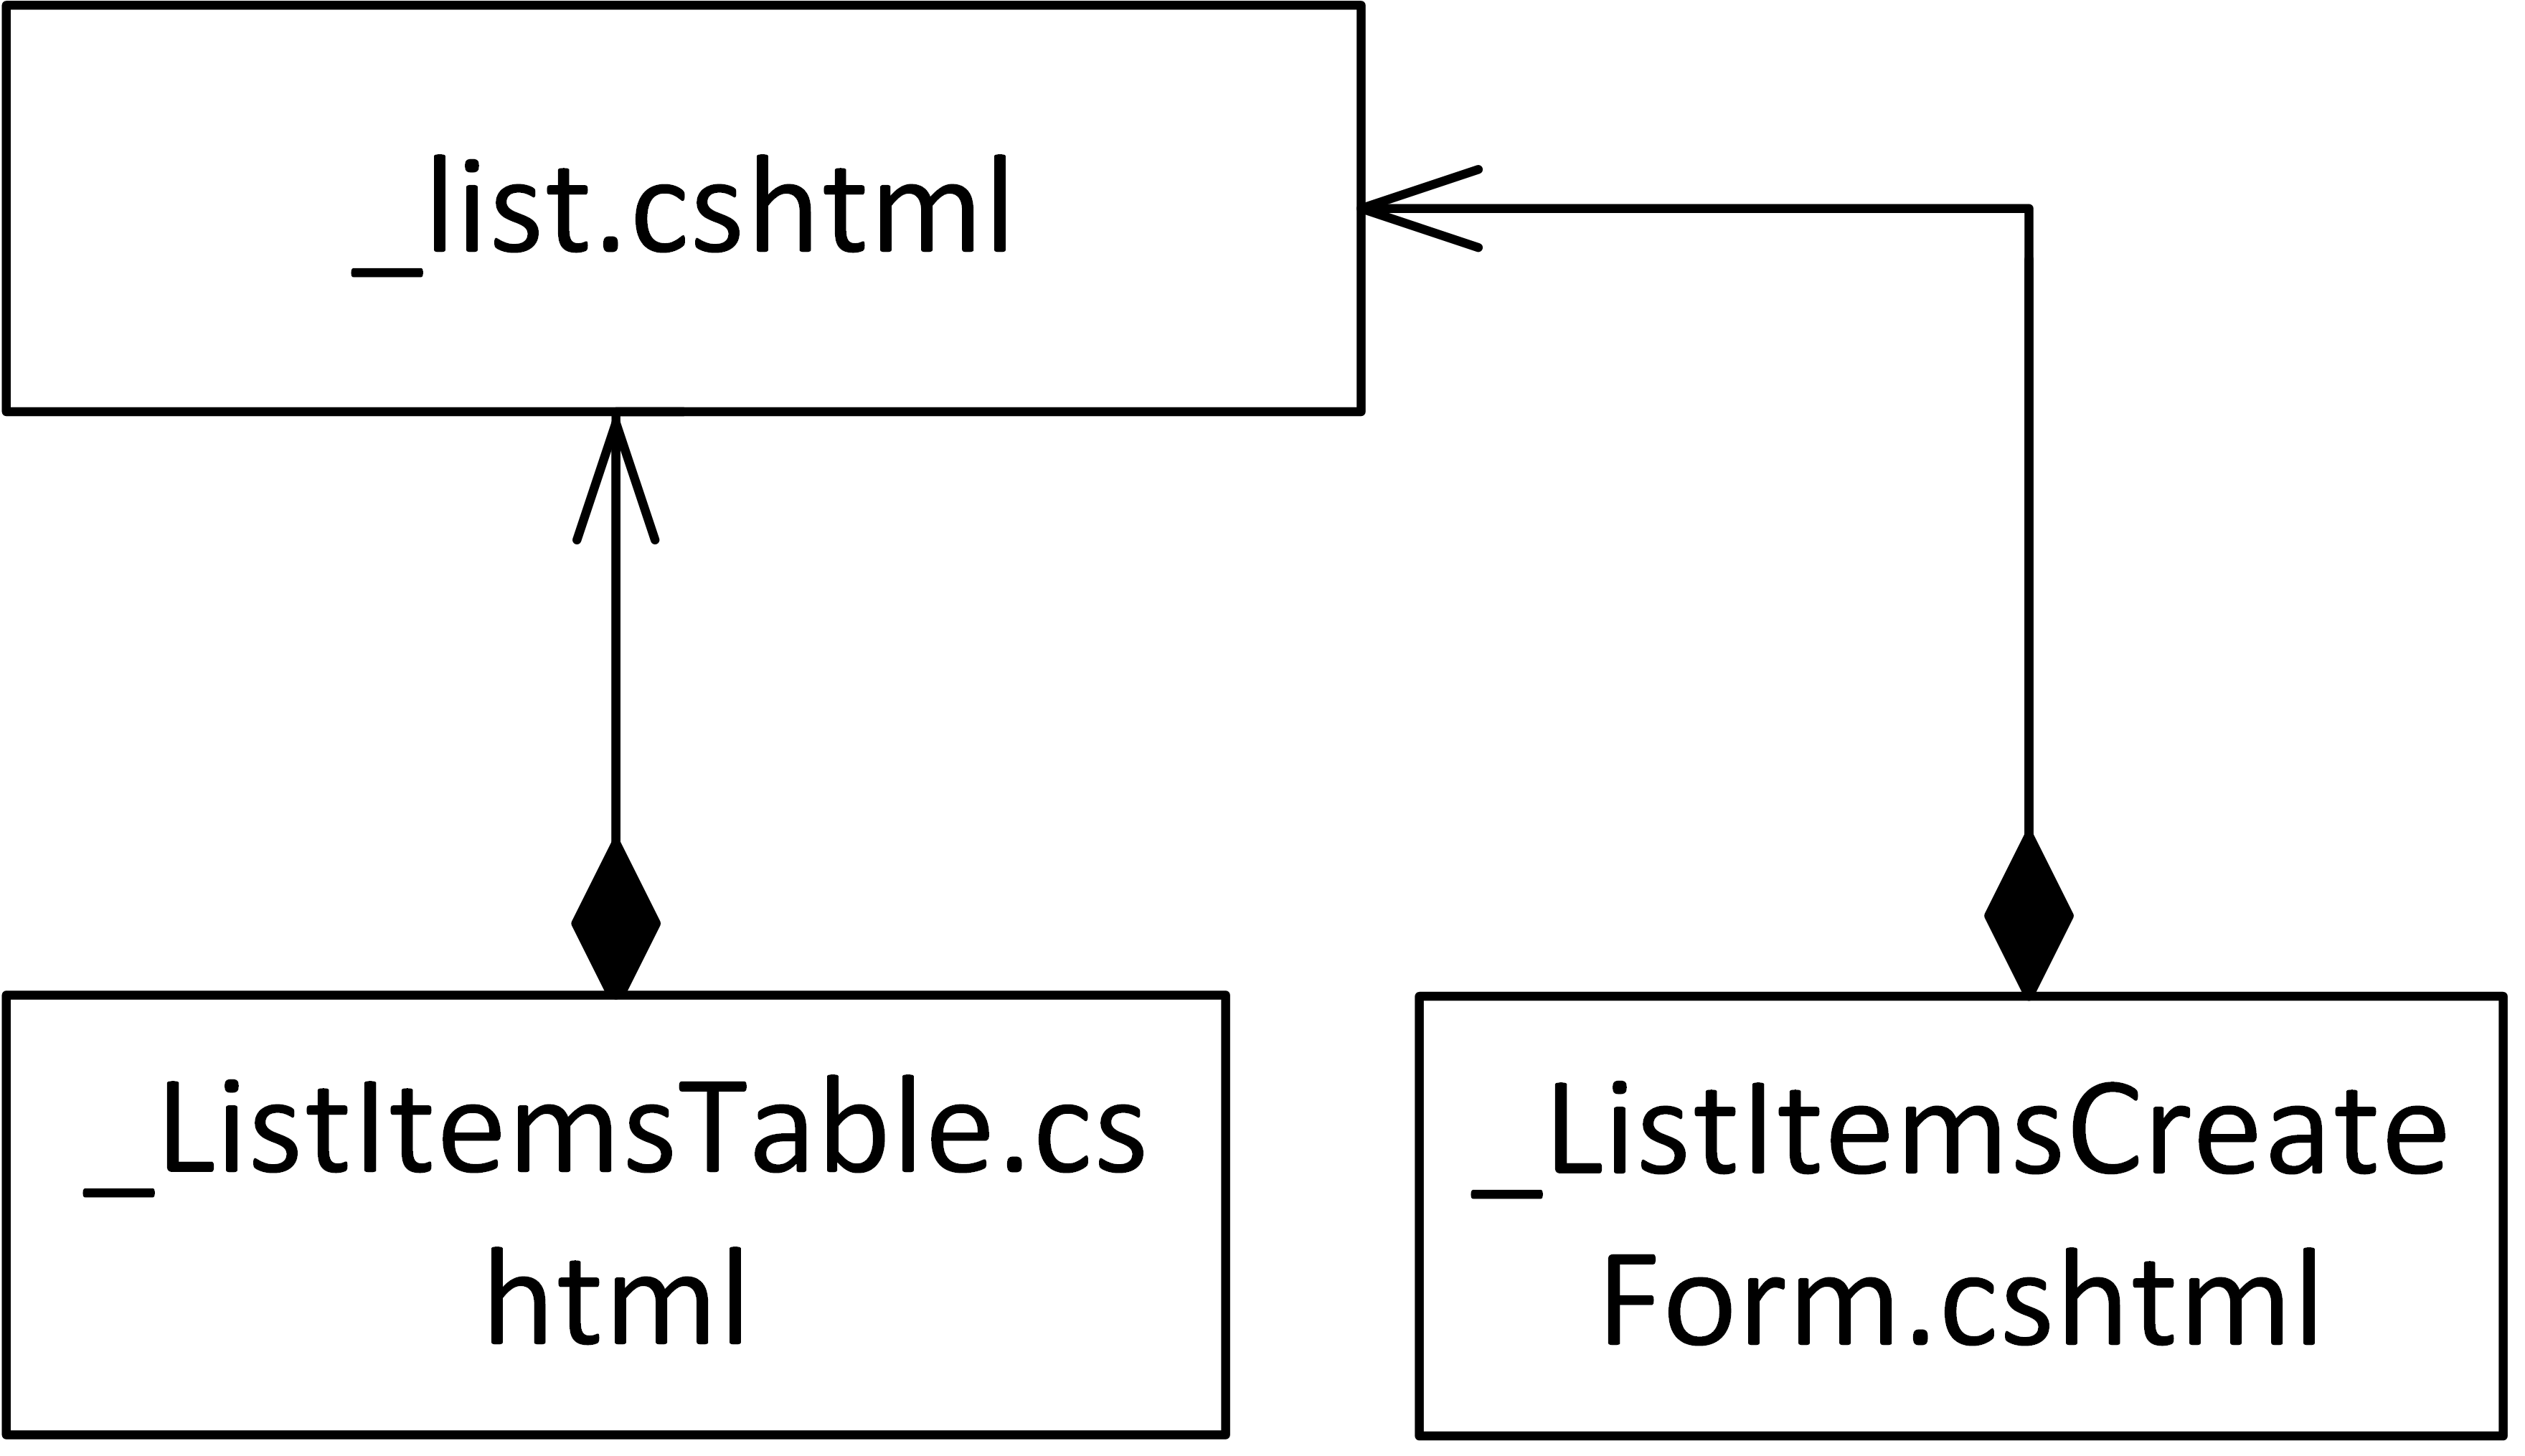
\includegraphics{10_Design_og_implementering/Lists/Images/list_composition.png}
    \caption{Her ses hvordan PartialViews er brugt inde i et andet PartialView. Det øverste er for selve Listen, hvor de 2 andre PartialViews bliver lavet. \_listItemsTable er den der lister alle ListItems og \_listItemsCreateForm er den der håndterer inputfeltet for at lave nye ListItems.}
    \label{fig:list_composition}
\end{figure}

\noindent Denne form for struktur er meget kendetegnet for MVC, som også tager brug af composite pattern, som betyder at der arbejdes i en træstruktur. Denne træstruktur er på samme måde anvendt i List, hvor der bliver brugt PartialViews inde i et PartialView.

\subsection{Implementering}

Ud fra krav til WePlanner er det defineret at en Widget af typen "List" skal have følgende funktionaliteter:

\begin{itemize}
    \item Afkrydsning/fjern afkrydsning af listeelementer
    \item Tilføj/slet liste elementer
    \item Tilføj \& rediger titel
    \item Slet alle afkrydsede listeelementer
\end{itemize}

Sådan som WePlanner er bygget op, har det været vigtigt at have muligeden for at lave lister, til at strukturere indkøb og andet der skal gøres. I en fremtidig iteration, ville list være mest optimal at tilgå list gennem en mobilvenlig formatering.

Ud fra arkitektur og design er List endt med at have følgende klassediagram. Udover actions i Controllerens er der lavet JavaScript, for at give brugervenligheden en chance for at være bedre.

\begin{figure}[H]
    \centering
    \includegraphics[width=\linewidth]{10_Design_og_implementering/Lists/Images/ListCDFinal.png}
    \caption{Klassediagrammet for List afspejler den funktionalitet der er angivet i Arkitekturen og Design af List. DAL for List er lavet med et interface, så dette kan fakes i integrationstests.}
    \label{fig:listCD}
\end{figure}

I ListController er mange actions blevet autogeneret, hvor de derefter er blevet modificeret til at passe til til WePlanner. Bl.a. bliver der stort set altid sendt et id med action. Dette kan være et widget id, gruppe id eller et listId. Udover de CRUD metoderne fra frameworket er der tilføjet yderligere metoder, som bliver kaldt med AJAX. Disse er POST's, som ændre noget i en liste.\\

\noindent Fx. ved funktionaliteten for at slette alle markerede list-elementer, bliver de først fjernet via JavaScript og derefter bliver Controller action ListItemsAjaxDeleteAllMarked(int? id) kaldt for at slette list-elementerne i databasen, hvor id er listId. Dem der skal slettes, er dem der har status for attributten IsDone $==$ true.